

\section{Options}

A \textbf{vanilla european call option} gives the right to buy something at a fixed price (the \textbf{strike}) in the future. If the future price is less than the strike price the option is worthless. You could exercise the option but you would only buy the thing for higher than the market price. If the future price is higher than the strike price the option has value: you can buy it for below market value, sell it at market value, and pocket the difference. 

That's what happens at expiry. Before expiry the option looks a little different. If the strike price is above the current price the option still has some value since it's possible that the price will increase before expiry. Before expiry the option price is a curvy function of the underlying price. 

 \begin{center}
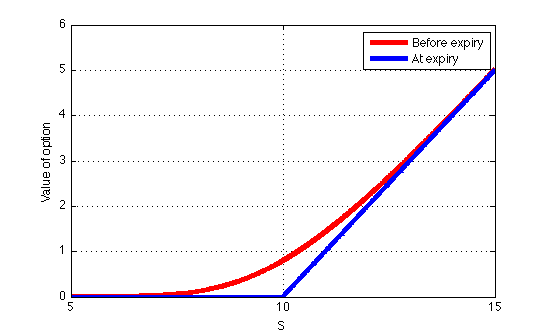
\includegraphics[width=4in]{pics/calltT}%
\captionof{figure}{Option value before and at expiry}\label{calltT}%
\end{center}

This curviness is the main characteristic of option portfolios. Managing a book of options is all about understanding and managing this curviness. 

\section{The problem}

We have a portfolio of \textbf{vanilla european options} on many underlying assets. We have two related tasks:

\begin{enumerate}
\item Determine the effect of changes in things that affect the options' values (e.g. underlying prices, time, implied volatilities, etc.). This is \textbf{simulation}.
\item Determine the contribution of these different things to a change in portfolio value after it has happened. This is \textbf{attribution}.
\end{enumerate}

Both can be tricky. Options are \textbf{non-linear} in most of the things that affect their price. A portfolio that is quite insensitive to price moves today might be very sensitive tomorrow. Worse, the things that drive options prices tend to be related to each other. Prices are related to implied volatilities, implied volatilities are related to interest rates, interest rates are related to everything. A portfolio of options can become a tangled web of these non-linear and sometimes surprising interactions. 

We'll try to untangle this web by breaking down portfolio value and sensitivity into bite-size chunks. Here we face a tradeoff: if the model is too simple we lose much of the relevant information; if the model is  too complicated it's difficult to interpret and likely to be misspecified. It's a gloomy situation for the portfolio manager but a rich and fascinating study for the student of options portfolio management.

Our approach is to start with the elements of option value and then look at the sensitivity of value to each element. Then we'll build methods to estimate the changes in value following from changes in these elements.


\section{Elements of option value}

We'll need some notation to start. The basic idea is that the value of an option derives partly from things that don't change (like the option strike and maturity), and partly from things that do change (like the underlying asset value and risk free rate). We have:

\begin{itemize}
\item $S_a(t)$ -- the price of some asset $a$ at time $t$\\
\item $r(T)$ -- the risk free interest rate for loans with maturity $T$\\
\item $O_{i_a}$ - the $i$'th option on asset $a$\\
\item $T_{i_a}$ -- the maturity of the $i$th option on asset $a$\\
\item $K_{i_a}$ -- the strike of the $i$th option on asset $a$\\
\item $\sigma_{i_a}$ The Black Scholes implied volatility for the $i$'th option on asset $a$\\
\item $\mathcal{F}_{i_a}$ -- the set of fixed things that determine the option value (e.g. strike, maturity) also called the \textbf{state variables}\\
\item $\mathcal{I}_{i_a}$ -- the set of changing things that determine the option value (e.g. implied volatility, asset price)\\
\end{itemize}

We use Black Scholes implied volatility purely as a quotation convention. We don't need to make any assumptions about how the asset behaves or even how the option is exercised. Yet. All that matters is there is a Black Scholes implied volatility for each asset, strike, and expiry.

In general the value of a particular option is a function of the fixed and varying components. 

\[V_{O_{i_a}} = V_{O_{i_a}}(\mathcal{F}_{i_a},\mathcal{I}_{i_a}) \]

The value of a portfolio of options sum up across assets and options

\[V = \sum_{a}\sum_{i_a}V_{O_{i_a}}(\mathcal{F}_{i_a},\mathcal{I}_{i_a}) \]

\section{Sensitivity}

Our first task is to determine the sensitivity  of each option to changes in the changing  elements. These are just the first derivatives of the value function with respect to the relevant variable

\[ \frac{\partial V_{O_{i_a}}}{\partial x}, x \in \mathcal{I}_{i_a}  \]

Each partial derivative has a name in options parlance. The most important sensitivities are

\begin{itemize}
\item $\frac{\partial V_{O_{i_a}}}{\partial S} $:  \textbf{Delta} -- sensitivity to change in underlying price\\
\item $\frac{\partial V_{O_{i_a}}}{\partial t} $: \textbf{Theta} -- sensitivity to change in time\\
\item $\frac{\partial V_{O_{i_a}}}{\partial \sigma_{i_a}} $:  \textbf{Vega} -- sensitivity to implied volatility\\
\item  $\frac{\partial V_{O_{i_a}}}{\partial r} $: \textbf{Rho} -- sensitivity to the risk free rate\\
\item $\frac{\partial^2 V_{O_{i_a}}}{(\partial S)^2} $: \textbf{Gamma} -- sensitivity of delta to change in the underlying price\\
\end{itemize}

These sensitivities are called \textbf{greeks} because some of them are named after greek letters, but they're not usually written as greek characters (write ``Delta'' rather than ``$\Delta$''). Some people do use capital greek letters to represent greeks but they run into trouble finding a sensible greek letter for `greeks' like \textbf{vega}, \textbf{vomma} (second order volatility sensitivity), and \textbf{zomma} (gamma sensitivity to volatility), which are not real greek letters. 
\subsection{Important greeks}

\subsubsection{Delta}

Delta is the sensitivity to the underlying price. For a single call option this is between 0 and 1. The delta is sometimes called the \textbf{hedge ratio} because it is the amount of the underlying you would need to hold to \textbf{hedge} the exposure of the option. An offsetting position in the underlying is called a \textbf{delta hedge}.
 
An old trader trick is to use the delta an estimate of the probability that the underlying will be above the strike at expiry. So if the delta is 0.25 there's around a 25\% probability that the option will end in the money.  This is only approximate but it's usually a good ballpark estimate.

\subsubsection{Theta}

Theta is the sensitivity to the passage of time. It is the change in the price of the option if time passes but nothing else changes. This is like the \textbf{yield} for a bond.

\subsubsection{Gamma}

This is the sensitivity of delta to the price. This is a very important greek because it determines the effectiveness of a hedge. If an option has a low gamma the change in value of the option will be similar to the change in value of a hedge (a linear position in the underlying). If an option has a high gamma the change in the value of the hedge will be different (since the correct value of the hedge is changing rapidly). 

Gamma for a call option can take any positive value. The gamma of an at-the-money option at expiry approaches infinity; the delta flicks between 0 and 1. This makes it difficult to manage gamma ahead of time. No matter how well you hedge there will always be scenarios where gamma approaches infinity.

Gamma is the bogey man for option traders. One moment they have a nice neatly delta hedged portfolio, the next the asset moves and the deltas stretch violently, making the hedge ineffective and exposing the portfolio to much higher risk. Many portfolios have died a gamma death. In the physical world gamma radiation (when energised atomic particles lose photons) will kill you; same in the financial world.

\subsection{What the greeks look like}

\begin{center}
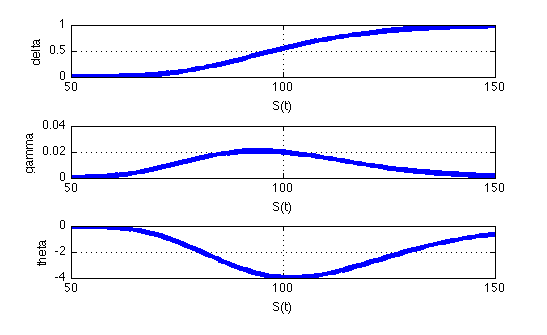
\includegraphics[width=5in]{pics/DeltaGammaTheta.png}
\captionof{figure}{Delta, Gamma and Theta for a call option}\label{DeltaGammaTheta}
\end{center}

Figure \ref{DeltaGammaTheta} has the value of delta, theta, and gamma for an at-the-money option as a function of the underlying asset (strike 100, implied volatility 0.2, expiring in 1 year, risk free rate is 0). Note two things in the figure: First, gamma changes with the slope of delta. Around the strike the delta changes most rapidly and so gamma  is highest, options deeply above or below their strikes have low gamma. Second, note that gamma and theta are negatively related. The relationship is captured in the saying ``good theta comes with bad gamma'' and can be shown explicitly for Black Scholes (with $r=0$)

\[ 0.5 S^2 \sigma^2 \mbox{Gamma} = -\mbox{Theta}\]

Don't worry about the derivation, the point is that theta and gamma are negatively related. . Figure \ref{DeltaGammaThetaT} shows the evolution of greeks for a particular evolution of $S(t)$ until the expiry of the option.

\begin{center}
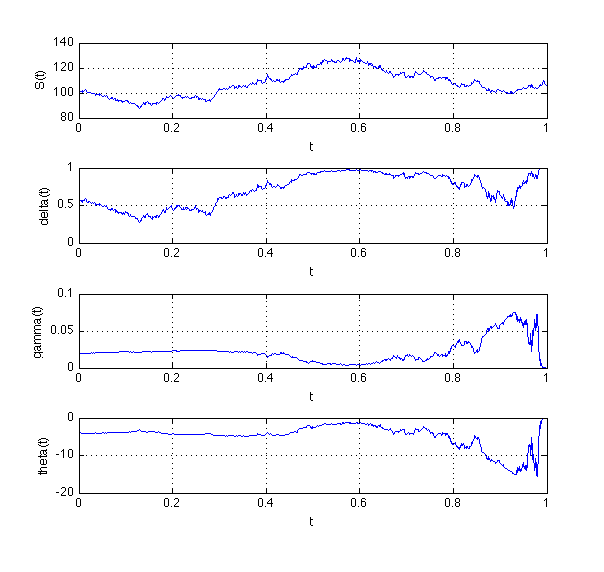
\includegraphics[width=5in]{pics/DeltaGammaThetaT.png}
\captionof{figure}{Delta, Gamma and Theta for a call option for a sample price path}\label{DeltaGammaThetaT}
\end{center}

The price path in figure \ref{DeltaGammaThetaT} was chosen randomly. The price starts at 100 and ends around 110, dipping above and below the strike. At little after t=0.8 the asset drops below the strike briefly and then recovers. Each greek has it's own story:


\textbf{The story of delta:}\\ Delta approaches zero when the call option is below the strike and 1 when it is above the strike. At the strike it is around 0.5.  The delta ends up at 1 since the asset ends above the strike. Between $t=0.6$ and $t=0.9$ when the asset approaches 100 the delta drops then recovers.\\
\textbf{The story of gamma:}\\ Gamma is high when the option is near to its strike. Around  $t=0.9$ gamma accelerates because the price is near to the strike and expiry is approaching. After t=0.95 the price runs away from the strike and gamma calms down, finally approaching zero since at expiry the option has no convexity.\\
\textbf{The story of theta:}\\ Theta does the opposite thing to gamma. This is because theta hates gamma.


\subsection{Dollar delta, dollar gamma, and dollar volatility}

If the underlying moves by $dS$ the value of the portfolio move is given by the Taylor series:

\begin{eqnarray*}
dV &= \underbrace{\frac{\partial V}{\partial S}dS}_{\mbox{dollar delta}} + \underbrace{\frac{1}{2}\frac{\partial^2 V}{(\partial S)^2 }(dS)^2}_{\mbox{dollar gamma}} + O((dS)^3) \\
 &\approx \mbox{ delta}*dS + \frac{1}{2}*\mbox{gamma}*(dS)^2
 \end{eqnarray*}

The first term is the \textbf{dollar delta}: the dollar amount that the value changes due to the delta. The second term is the \textbf{dollar gamma}: the amount the dollar value changes due to the delta. The sum of the two terms is a pretty good approximation of the effect of a change in the underlying (you can always add higher order terms if you want more accuracy). If the portfolio is delta hedged the dollar delta is offset and you're left with the dollar gamma (and higher order terms).  An option delta hedged to expiry is exposed  to the sum (integral) of all the dollar gammas at each point in time.

\subsubsection{Dollar volatility}
Dollar delta and dollar gamma are great but they involve an unknown term $dS$.  A sensible choice for $dS$  is the implied volatility multiplied by the spot price $ \sigma S$. The idea is that a one standard deviation movement in the underlying will be $S\sigma$ (if volatility is priced correctly). The effect on the options price is this multiplied by the option's delta. This is a good first-pass way to measure and compare risks across different options and option portfolios. 

We could develop more dollar greeks (dollar vega is popular) but the point is served with these few. In any case we'll be developing a full Taylor series with all dollar sensitivities and cross terms a little later. 

\section{Simulation, perturbation, and attribution}

\subsection{Breaking it down}

Remember that we're doing all this to achieve two things: First, we want to \textbf{simulate} the effect of some move in the option pricing variables on the value of the portfolio.

 Second, we want to \textbf{attribute} changes in prices to different factors. 
 
For both we can use a \textbf{first principles} approach, revaluing the total option portfolio with a pricing formula, or a \textbf{perturbation} approach, building a Taylor series and estimating effects for the first (usually) two terms. We'll develop both methods and work through a few examples.

\subsection{First principles or perturbation?}

We can simulate the effect of a change in the \textbf{state variables} either by repricing the whole portfolio under the old and new state variables (\textbf{first principles}) or by using a Taylor series (\textbf{perturbation}). The advantage of the first principles approach is that it's more precise, the advantage of the perturbation approach is that it's more transparent. With a Taylor series we  decompose the marginal first and second order effects of movements in the state variables. If we were really clever this wouldn't be an advantage; we'd be able to see the effect of any change in the state variables just by looking at the pricing equation. It's only because we're not this clever (sorry, but I'm speaking for both of us) that a perturbation approach is helpful.

\subsubsection{Breaking it down}

If the state variables change from $\mathcal{I}$ to $\mathcal{I'}$ the change in portfolio value is

\[ \Delta V =  \sum_{a}\sum_{i_a}V_{O_{i_a}}(\mathcal{F}_{i_a},\mathcal{I'}_{i_a}) - \sum_{a}\sum_{i_a}V_{O_{i_a}}(\mathcal{F}_{i_a},\mathcal{I}_{i_a})  \]
 
 This means we reprice the portfolio with the new state variables and take the difference. For a change in a \textit{particular} state variable $I \in \mathcal{I}$ the perturbation approach uses a Taylor series
 
 \[ \Delta V  = \sum_{a}\sum_{i_a}  \left(  \frac{ \partial V_{O_{i_a}}}{\partial I}(I-I') + \frac{1}{2}\frac{\partial^2 V_{O_{ia}}}{(\partial I)^2}(I-I')^2 + O((I-I')^3)  \right)  \]

(as usual we'll ignore everything after the second term) To make things easy we can assume that the first and second order sensitivities are zero if $I \notin \mathcal{I}_{ia}$. So, for instance, the sensitivity of an option on company $A$ to a movement in company $B$'s stock price is zero. If we're being more adventurous we can allow these sensitivities to be nonzero, but then we have to use a multivariate Taylor series, and that's a little more complicated. You can do it if you like but I'm going to do something else.

\subsubsection{Example}

Say we have a portfolio of four call options, two each on corn and wheat. The spot price of corn is $S_C(0) = 100$ and wheat $S_W(0) = 200$. Assume that all risk free rates are zero. Assuming everything is priced by standard Black-Scholes with a risk free rate of 0 and no dividends the options look like this:

\begin{tabular}{|c|c|c|c|c|}
\hline
Underlying & Expiry & Strike & Implied volatility & Price\\ 
\hline
Corn ($C1$) & 1 & 100 & 0.2 & 7.97 \\
Corn ($C2$) & 2 & 100 & 0.2& 11.24 \\
Wheat ($W1$) & 1 & 200 & 0.3& 22.85 \\
Wheat ($W2$)  & 2 & 200 & 0.3& 33.60  \\
\hline
\end{tabular}

We name the options C1, C2, W1, and W2 after their underlings and maturities. 

Our dollar greeks (per option) are:

\begin{tabular}{|c|c|c|c|c|}
\hline
Option & Dollar delta & Dollar gamma & Dollar theta & Dollar vega\\ 
\hline
Corn ($C1$) & 0.54*dS & $0.5*\mbox{gamma}*(dS)^2 = 0.0099*(dS)^2 $ & $-3.96*dt$ & $39.69*d\sigma$ \\
Corn ($C2$) & 0.56*dS & $0.0070*(dS)^2$ & $-2.79*dt$& $55.86*d\sigma$ \\
Wheat ($W1$) & 0.56*dS & $0.0033*(dS)^2$ & $-11.83*dt$ & $78.90*d\sigma$ \\
Wheat ($W2$) &  0.58*dS & $0.0023*(dS)^2$ & $-8.27*dt$ & $110.32*d\sigma$ \\
\hline
\end{tabular}

This table tells us a lot.

\begin{itemize}
\item  All options move a little more than 0.5 for every \$1 move in the underlying. 
\item  Gamma is lower for options with longer maturities. (because function is less convex)
\item Theta is lower for options with longer maturities. The daily yield on the first wheat option is $-11.83*1/365 = 0.0324$ or 0.14\% of the price.  Annualised this is 51.77\% of the price. Not bad. 
\item Vega is pretty large. A 0.01 increase in implied volatility increases the option price by more than 3\%
\end{itemize}

%We don't often look at their second order sensitivities for theta and vega because both are relatively linear. For volatility and time the first order approximation is a pretty good estimate of the true change in value, particularly for vega.

We can now simulate some events. If the price of corn rises by \$10 overnight the change in the portfolio will be (by the two-term Taylor series)

\[ \Delta V \approx \underbrace{0.54*10}_{\mbox{C1 dollar delta}}+\underbrace{0.0099*10^2}_{\mbox{C1 dollar gamma}}+  \underbrace{0.56*10}_{\mbox{C2 dollar delta}}+\underbrace{0.0070*10^2}_{\mbox{C2 dollar gamma}} = 12.69  \]

This is quite substantial given that the combined value of the two options is less than 20 at the start. Good to know.

If implied volatility for corn jumps up by 0.1 to 0.2  we get

\[\Delta V  \approx 6.68*0.1+55.86*0.1 = 9.25 \]

Again, a big move.

For a little more texture we'll consider five examples. In each we'll construct the first principles and perturbation equations. The first two are for simple changes for one underlying. The third example constructs the equation if the prices of wheat and corn are related. In the fourth example the implied volatility is related to the strike price.  We'll see that strange things happen with interactions: If the underlying price and the implied volatility move together the marginal effect of the price increase will be different depending on which is calculated first. 


\medskip
\textbf{Example 1: Pure price increase}\\

If the price of corn increases by 10 we can calculate the new option prices directly
\medskip

\begin{tabular}{|c|c|c|c|c|c|c|}
\hline
Underlying & Expiry & Strike & Implied volatility & Strike' & Implied volatility' & $\Delta V$\\ 
\hline
Corn & 1 & 100 & 0.2 & \textbf{110} & 0.2 &\textbf{ 6.33} \\
Corn & 2 & 100 & 0.2& \textbf{110} & 0.2 & \textbf{6.22} \\
Wheat & 1 & 200 & 0.3& 200 & 0.3 & 0\\
Wheat & 2 & 200 & 0.3& 200 & 0.3 &  0\\
\hline
\end{tabular}

\medskip

or approximate with a Taylor series:

\begin{eqnarray*}
\Delta V_{C1} \approx \mbox{dollar delta + dollar gamma} = 0.54 dS + 0.0099*(dS)^2 = 0.54*10+0.0099*10^2 = 6.39\\
\Delta V_{C2} \approx \mbox{dollar delta + dollar gamma} = 0.56 dS + 0.0070*(dS)^2= 0.56*10+0.0070*10^2 = 6.3\\
\end{eqnarray*}

\textbf{Example 2: Pure volatility curve shift}\\

If all implied volatilities increase by 0.1 the price movements are

\begin{tabular}{|c|c|c|c|c|c|c|}
\hline
Underlying & Expiry & Strike & Implied volatility & Strike' & Implied volatility' & $\Delta V$\\ 
\hline
Corn & 1 & 100 & 0.2 & 100& \textbf{0.3} & \textbf{3.96} \\
Corn & 2 & 100 & 0.2& 100 & \textbf{0.3} & \textbf{5.55} \\
Wheat & 1 & 200 & 0.3& 200 & \textbf{0.4} & \textbf{7.86} \\
Wheat & 2 & 200 & 0.3& 200 & \textbf{0.4} & \textbf{10.94}  \\
\hline
\end{tabular}

For the Taylor series we only use the first term because price is fairly linear in volatility. 

\begin{eqnarray*}
\Delta V_{C1} \approx \mbox{dollar vega}  = 39.69 d\sigma  = 39.69 *0.1 = 3.97\\
\Delta V_{C2} \approx \mbox{dollar vega}  = 55.86 d\sigma  = 55.86 *0.1 = 5.59\\
\Delta V_{W1} \approx \mbox{dollar vega} = 78.90 d\sigma = 78.90*0.1 = 7.89\\
\Delta V_{W2} \approx \mbox{dollar vega} = 110.32 d\sigma = 110.32*0.1 = 11.32
\end{eqnarray*}

The approximation would be slightly better if we used the second order volatility (dollar vomma). But we won't, partly in protest against the silly name. 

\textbf{Example 3: Wheat and corn prices related}

Say that wheat and corn prices are related by a function $S_W = S_C-100$. If the price of corn rises by 10 then the price of wheat also rises by 10:

\begin{tabular}{|c|c|c|c|c|c|c|}
\hline
Underlying & Expiry & Strike & Implied volatility & Strike' & Implied volatility' & $\Delta V$\\ 
\hline
Corn & 1 & 100 & 0.2 & \textbf{110} & 0.2 & \textbf{6.33} \\
Corn & 2 & 100 & 0.2& \textbf{110} & 0.2 & \textbf{6.22} \\
Wheat & 1 & 200 & 0.3& \textbf{210} & 0.3 & \textbf{5.91} \\
Wheat & 2 & 200 & 0.3& \textbf{210} & 0.3 & \textbf{6.06}  \\
\hline
\end{tabular}

We can calculate the effect by substituting $dS = 10$ into the Taylor Series for Corn and Wheat

\begin{eqnarray*}
\Delta V_{C1} \approx \mbox{ dollar delta + dollar gamma} = 0.54*dS + 0.0099*(dS)^2 = 0.54*10+0.0099*10^2 = 6.39\\
\Delta V_{C2} \approx \mbox{dollar delta + dollar gamma} = 0.56*dS + 0.0070*(dS)^2= 0.56*10+0.0070*10^2 = 6.3\\
\Delta V_{W1} \approx \mbox{dollar delta + dollar gamma} = 0.56*dS + 0.0033*(dS)^2 = 0.56*10+0.0033*10^2 = 5.93\\
\Delta V_{W2} \approx \mbox{dollar delta + dollar gamma} = 0.58*dS + 0.0023*(dS)^2= 0.58*10+0.0023*10^2 = 6.03\\
\end{eqnarray*}


\textbf{Example 4: Volatility is a function of price}

Now let's say that volatility is a function of the price by the function $\sigma_{C} = -0.001*S_C+0.3$. If the spot price of corn is 100 then the volatility is $-0.001*100+0.3 = 0.2$, If the price moves to 100 the volatility becomes $-0.001*100+0.3 = 0.19$. We can see the joint effect by repricing both corn and corn implied volatility:

\begin{tabular}{|c|c|c|c|c|c|c|}
\hline
Underlying & Expiry & Strike & Implied volatility & Strike' & Implied volatility' & $\Delta V$\\ 
\hline
Corn & 1 & 100 & 0.2 & \textbf{110} & \textbf{0.19} & \textbf{5.96} \\
Corn & 2 & 100 & 0.2& \textbf{110} & \textbf{0.19} & \textbf{5.67} \\
\hline
\end{tabular}

The approximation is constructed by combining the approximate effects of the move in underlying price (dollar delta + dollar gamma) and in implied volatility (dollar vega):

\begin{eqnarray*}
\Delta V_{C1} &\approx \mbox{dollar delta + dollar gamma + dollar vega} = 0.54*dS + 0.0099*(dS)^2 + 39.69*d\sigma \\
 &= 0.54*10+0.0099*10^2 + 39.69*(-0.01) =  5.99\\
\Delta V_{C2} &\approx \mbox{dollar delta + dollar gamma + dollar vega} = 0.56*dS + 0.0070*(dS)^2 + 55.86*d\sigma\\
 &= 0.56*10+0.0070*10^2 + 55.86*(-0.01) = 5.74\\
%\Delta V_{W1} \approx dollar delta + dollar gamma + dollar vega = $0.56*dS + 0.0033*(dS)^2 + 78.90*d\sigma$ = $0.56*10+0.0099*10^2 + 78.90*(-0.01)$ = 5.93\\
%\Delta V_{W2} \approx dollar delta + dollar gamma + dollar vega = $0.58*dS + 0.0023*(dS)^2 + 110.32*d\sigma$= $0.58*10+0.0070*10^2 + 110.32*(-0.01)$ = 6.03\\
\end{eqnarray*}

This give the \textit{total} effect. If we want the \textbf{marginal} effect we have to change one thing at a time. Because the pricing function is nonlinear the estimated marginal effects will depend on which move we do first. 

If the price moves first we have:

\begin{tabular}{|c|c|c|c|c|c|c|}
\hline
Underlying & Expiry & Strike & Implied volatility & Strike' & Implied volatility' & $\Delta V$\\ 
\hline
Corn & 1 & 100 & 0.2 & \textbf{110} & 0.2 & \textbf{6.33} \\
Corn & 2 & 100 & 0.2& \textbf{110} & 0.2 & \textbf{6.22} \\
\hline
\end{tabular}

Then move the volatility given that the price has moved:

\begin{tabular}{|c|c|c|c|c|c|c|}
\hline
Underlying & Expiry & Strike & Implied volatility & Strike' & Implied volatility' & $\Delta V$\\ 
\hline
Corn & 1 & 110 & 0.2 & 110 & \textbf{0.19} & \textbf{-0.37} \\
Corn & 2 & 110 & 0.2& 110 & \textbf{0.19} & \textbf{-0.55} \\
\hline
\end{tabular}

Now try moving the volatility first:

\begin{tabular}{|c|c|c|c|c|c|c|}
\hline
Underlying & Expiry & Strike & Implied volatility & Strike' & Implied volatility' & $\Delta V$\\ 
\hline
Corn & 1 & 100 & 0.2 & 100 & \textbf{0.19} & \textbf{-0.40} \\
Corn & 2 & 100 & 0.2& 100 & \textbf{0.19} & \textbf{-0.56} \\
\hline
\end{tabular}

Notice that the marginal effect is different. When volatility moves first the effect on the $C1$ is 0.4 but when price moves first it's 0.37. 

Now move the price:

\begin{tabular}{|c|c|c|c|c|c|c|}
\hline
Underlying & Expiry & Strike & Implied volatility & Strike' & Implied volatility' & $\Delta V$\\ 
\hline
Corn & 1 & 100 & 0.19 & \textbf{110} & 0.19 & \textbf{6.35} \\
Corn & 2 & 100 & 0.19& \textbf{110} & 0.19 & \textbf{6.23} \\
\hline
\end{tabular}

Again the marginal effect is different. If price move first the effect on $C1$ is 6.35 compared to 6.33 when volatility moves first. 

There is no correct order to view marginal effects in these types of problems. For the full calculation it doesn't matter because it comes out the same each way. But it would be nice to be able to identify precisely which effect was which. Nice, but impossible.

%(note that volatility is more commonly a function of delta with ATM smallest

\section{A general schema for options portfolio management}

The basics are:

\begin{enumerate}
\item An option's value depends on some \textbf{fixed things} (like the strike and expiry) and on \textbf{variable things} (like the underlying asset price,  and implied volatility).
\item The sensitivity of options to changes in the variable things are called the \textbf{greeks}:
\begin{itemize}
\item The first order sensitivity to underlying price is called \textbf{delta}. Delta is bounded between 0 and 1.\\
\item The second order sensitivity to underlying price is called \textbf{gamma}. Gamma is unbounded above and can approach infinity for an at the money option close to expiry.\\
\item The first order sensitivity to implied volatility is called \textbf{vega}\\
\item The first order sensitivity to time is called \textbf{theta}\\
\end{itemize} 
\item None of the greeks should be written as a greek letter. Especially vega because it isn't a real greek letter.
\item The \textbf{dollar greeks} are estimates of the total dollar effect of a change in the variables. For most variables this is just the greek multiplied by the change in the variable. For \textbf{dollar gamma} it's the entire second term of the \textbf{Taylor series}: $\frac{1}{2}\mbox{Gamma}*dS^2$\\
\item The effect of changes in the variable things can be estimated from \textbf{first principles} (by repricing the option with the new variables) or by \textbf{perturbation} (by building a Taylor series approximation of the price and taking the first one or two terms).
\end{enumerate}

The value of option $i$ on asset $a$ is

\[V_{O_{ia}}(\mathcal{F}_{i_a},\mathcal{I}_{i_a}) \]

The value of a portfolio of options on multiple assets is

\[V = \sum_{a}\sum_{i_a}V_{O_{i_a}}(\mathcal{F}_{i_a},\mathcal{I}_{i_a}) \]

For a change in a \textit{particular} state variable $I \in \mathcal{I}$ the change in portfolio value from \textbf{first principles} is

\[ \Delta V =  \sum_{a}\sum_{i_a}V_{O_{i_a}}(\mathcal{F}_{i_a},\mathcal{I'}_{i_a}) - \sum_{a}\sum_{i_a}V_{O_{i_a}}(\mathcal{F}_{i_a},\mathcal{I}_{i_a})  \]

This can be used to model any sequence of changes in all state variables. 
 
 the \textbf{perturbation approach} uses a Taylor series:
 
 \[ \Delta V  = \sum_{a}\sum_{i_a}  \left(  \frac{ \partial V_{O_{i_a}}}{\partial I}(I-I') + \frac{1}{2}\frac{\partial^2 V_{O_{i_a}}}{(\partial I)^2}(I-I')^2 + O((I-I')^3)  \right)  \]
 
 For instance for a change in the underlying price the perturbation equation is

 \[ \Delta V  = \sum_{a}\sum_{i_a}  \left(  \mbox{delta}*dS + \frac{1}{2}\mbox{gamma}*dS^2 + O(dS^3)  \right)  \]

If the state variables are related to each other (for instance if volatility is a function of the underlying price) then we can sum the equation for the original state variable $I$ and the equation for the other affected state variables.

\subsection{Stress testing}

It's useful to know how an options book would perform in extreme market events. Simulating this is very simple: first specify how some extreme event would affect the state variables (particularly underlying price and implied volatilities). One approach is to look at historical market move during some extreme event like a market crash. Then plug these changes into the first principles pricing equation. For extra marks sample from a \textbf{joint probability distribution} of state variables and create a distributional estimate of portfolio value under the extreme scenario. 

\section*{Questions}

\textbf{Question 1:}

An asset is currently priced at 100. The implied volatility for any option is given by the function

\[ \sigma_K =  0.2 +  \frac{(K-S)^2}{10000} \]

where $K$ is the strike price and $S$ the asset price. We have a portfolio of two call options with the following specifications and greeks


\begin{center}
\begin{tabular}{|c|c|c|}
\hline
 & Option 1 & Option 2\\
 \hline
 Strike & 93 & 103.1\\
 Delta & 0.4 & 0.6\\
 Gamma & 0.0187 & 0.0203\\
 Vega & 39.85 & 39.95\\
 Theta & -4.0 & -3.68\\
\hline
\end{tabular}
\end{center}

\begin{itemize}
\item[(a)] The underlying moves instantaneously to 110. Estimate the total effect on portfolio value using a Taylor series.
% delta1*10 + 0.5*gamma1*(10)^2 + vega1*d sigma1 etc. (sigma 1 and sigma 2 calculated by the function)
\item[(b)] Suppose that we also have a short position in one unit of the asset (this gains \$1 for each \$1 decrease in the asset). What approximate change in the asset value (starting at 100) would leave the portfolio value unchanged after 1 day
% Set 0.5*gamma1*(dS)^2 + vega1*d sigma1 + theta1*(1/365) = 0 and solve for dS (not e that d sigma1 can be written as a fn of dS )

\end{itemize}


\section*{Appendix: Taylor series}

A continuous function $f(x)$ centred at $a$ is approximated by the \textbf{Taylor series}

\[f(x) = f(a) + \frac{f'(a)}{1!}(x-a) + \frac{f''(a)}{2!}(x-a)^2 + \frac{f(3)(a)}{3!}(x-a)^3 + \ldots  \]

where $f^n(a)$ is the $n$'th derivative of the function. For example the function $x^3$ around $a$ is  

\[f(x) = a^3 + \frac{3a^2}{1!}(x-a)  + \frac{4a}{2!}(x-a)^2 + \frac{4}{3!}(x-a)^3\]

Around 2 this is

\begin{eqnarray*}
f(x) &= 2^3 + \frac{3*2^2}{1!}(x-2)  + \frac{6*2}{2!}(x-2)^2 + \frac{6}{3!}(x-2)^3 \\
 &= 2^3 + 12*(x-2) + 6*(x-2)^2 + (x-2)^2
\end{eqnarray*}

Now say we want to know f(4). We plug in 4 to the series:

\[2^3 +12*(4-2) + 6*(4-2)^2 + (4-2)^3 = 64\]
 
 Marvellous. We now have a very complicated way to find $4^3=64$. But why stop there? 
 
 We want an expression for the \textbf{change} in the value of the function around some point. We substitute $(x-a) = dx$ and rearrange the Taylor series to get our answer:
 
 
 \begin{eqnarray*}
 f(x) = f(a) + \frac{f'(a)}{1!}(x-a) + \frac{f''(a)}{2!}(x-a)^2 + \frac{f(3)(a)}{3!}(x-a)^3 + \ldots  \\
df(x) =f(a+dx) -  f(a)  =  \left(\frac{f'(a)}{1!}(dx) + \frac{f''(a)}{2!}(dx)^2 + \frac{f^3(a)}{3!}(dx)^3 + \ldots \right) 
\end{eqnarray*}

For example the change in the function $x^3$ around 3 is

\begin{eqnarray*}
3x^2(dx) + \frac{6x}{2!}dx^2 + \frac{6}{3!}dx^3\\
3*3^2(dx) + \frac{6*3}{2!}dx^2 + \frac{6}{3!}dx^3
\end{eqnarray*}


for $dx=1$ the change is 37. This is also $4^3-3^3 = 64-27$.

\subsection*{Higher order Taylor series and big O notation}
With $x^3$ the Taylor series only has 4 terms before the function runs out of derivatives. Many functions never run out of derivatives so the Taylor series go on forever. Forever is too long to spend writing out Taylor series so sometimes we ignore terms after a point. This works if the higher order terms are smaller, which is true for many common functions. When we truncate the series we add in a term at the end to represent the rest:

\[df(x) =f(a+dx) -  f(a)  =\frac{f'(a)}{1!}(dx) + \frac{f''(a)}{2!}(dx)^2 + \frac{f^3(a)}{3!}(dx)^3 + O(dx^4)\]

The final term $O(dx^4)$ means that all the terms after are smaller than some constant times $dx^4$.  If we're satisfied that these are sufficiently small we ignore them.



